% vim:set et sw=2 ts=4 tw=72:

\section{Design and Implementation}
\label{sec:design}

We constructed a web-based tool called \tool in order to navigate and
inspect the \mt visualizations of the kernel. Creating the web-based
tool enables users to use the system without having to install
additional software or store a large database, which makes it more
accessible, easily maintainable, and platform independent. \tool uses
the following mechanisms to reach our goals of better navigation and
better explanation of the selected changes.

\begin{itemize}
        \item Filter by searching
        \item View aggregated summaries of authors, files, and modules
        \item Visualize \mt{s}
\end{itemize}

\subsection{Search}

\tool provides a search engine for navigating within the kernel,
filtering commits that are not relevant. The search engine takes a
plain text query from the user and returns the results that are relevant
in the order of relevancy. When computing relevancy, the engine uses the
commit log, the author name, the filenames, the commit hash, the date
the commit was authored, and the date the commit was committed.

\begin{figure}[htpb]
  \centering
  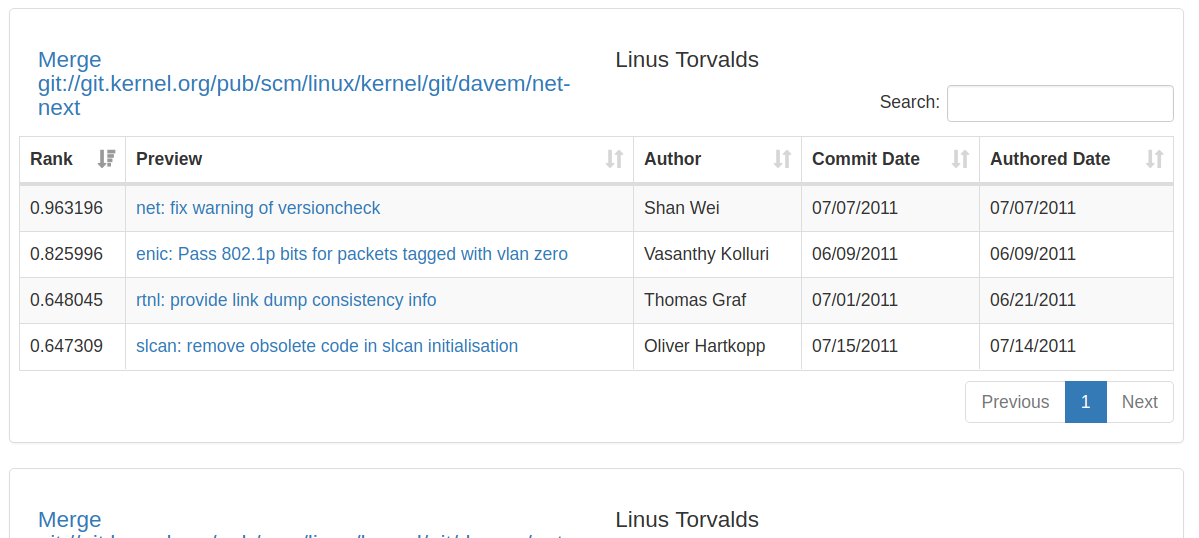
\includegraphics[width=\figwidth]{figures/linvis/search_results.png}
  \caption{A single \mt tree in the search results of \tool, showing
    the link to the root at the top and a table of the relevant commits
    in the bottom, sorted by relevance.}
  \label{fig:search_results}
\end{figure}

Before presentation, the results are grouped by \mt root. Each group
has a link to the root-node of the tree at the top, followed by a table
of commits and merges within the tree that match the query, shown in
Figure~\ref{fig:search_results}. The table includes the relevancy rank
of the entry, the commit log message preview, author, the date the
repository event was committed, and the date it was authored. The merge
tree groups are ordered based on the mean of the relevancy scores of the
relevant results in that tree.

\subsection{Summarization}
\label{sub:summarization}

\tool uses seven tabs to show the information and visualizations for a
selected repository event. The summarization tabs are; messages, files, modules,
authors; the visualization tabs are; list tree, pack tree, and \rt tree.

The message tab shows the full commit log message. This does not include
the diff, but given the commit hash, this information can be found
directly from the repository.

The files tab shows an aggregated table of all files that were modified
in a merge. It includes metrics like the number of lines added, lines
removed, total lines modified, and the delta, summed across all commits
in the \mt tree that modify this file. A details drop-down button
allows a user to see exactly which commit makes the changes, as shown in
Figure~\ref{fig:linvis_files}. If the current repository event being
viewed is a commit, the aggregate views will only show modifications
made by the commit.

The modules tab shows the modules modified in the \mt. Like the
files tab, the modules tab uses a table to show the name of the module,
the number of commits that are in the \mt tree that work with the
module, and a details button to provide the links to those commits.

\begin{figure}[htpb]
  \centering
  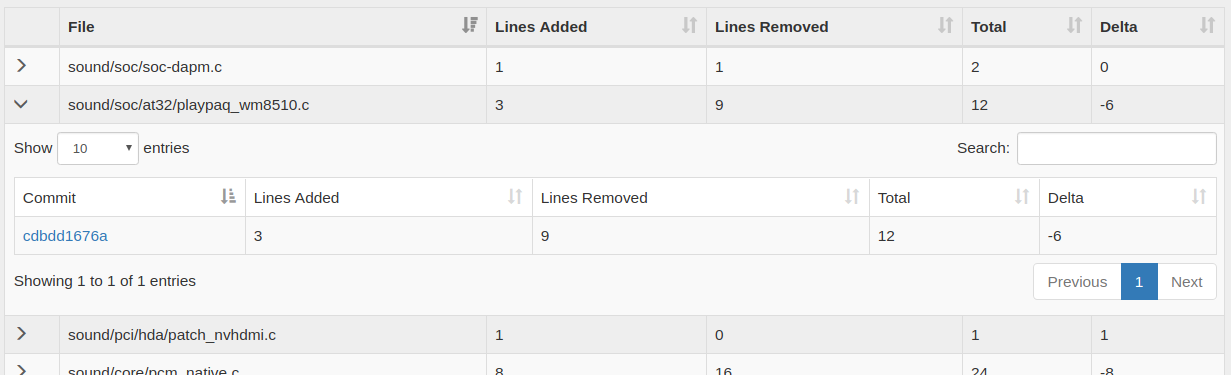
\includegraphics[width=\figwidth]{figures/linvis/linvis_files.png}
  \caption{Table showing the modified files in a merge, with the second
  entry expanded to show the commit that makes the changes.}
  \label{fig:linvis_files}
\end{figure}

The authorship tab is very similar to the files tab, but shows the
authorship information. It shows the sum of the number of lines added,
removed, modified, and the delta within the \mt. It also shows the
number of files that were modified by the author. The details tab is
organized slightly differently. Instead of organizing the results by
commit, the details are organized by file, showing which files were
modified by the author in this \mt (Figure~\ref{fig:linvis_authors}).

\begin{figure}[htpb]
  \centering
  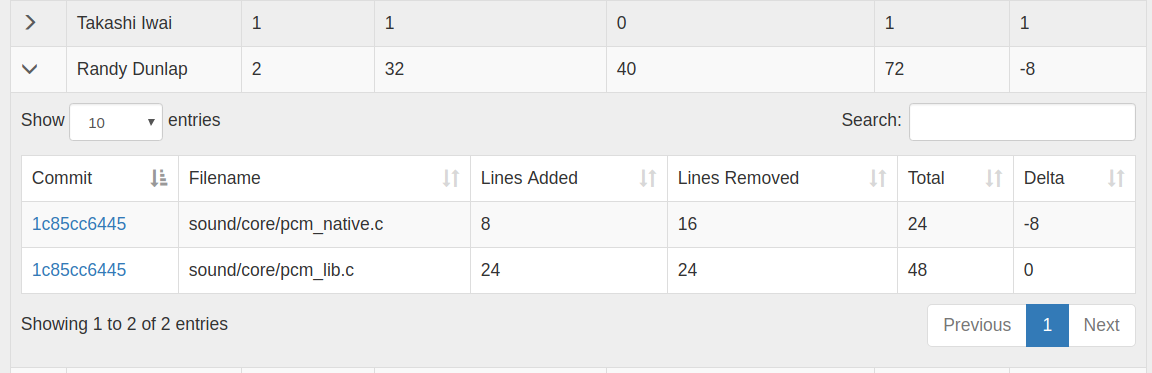
\includegraphics[width=\figwidth]{figures/linvis/linvis_authors.png}
  \caption{Table showing the authors who made changes in a merge. The
    entry for Randy Dunlap is expanded, showing the modifications to
    each file that were made by Randy.}
  \label{fig:linvis_authors}
\end{figure}


\subsection{Visualization}
\label{sub:visualization}

The ability to easily visualize the integration of commits into a
project is what makes \tool unique from other tools. \tool implements
three visualizations, the list tree, pack tree, and \rt tree.

\subsubsection{List Tree}

The list tree, depicted in Figure~\ref{fig:linvis_list_tree}, is
constructed as a series of nested lists. The nesting indicates the
parent-child relationship. This visualization is text-based enabling
fast navigation to commits using the built-in search in most
web-browsers. The list tree is rooted at the current repository event;
if the current event being inspected is a commit, only that commit will
be shown. Conversely, if the selected event is the root, the entire
\mt tree will be shown.

\begin{figure}
        \centering
        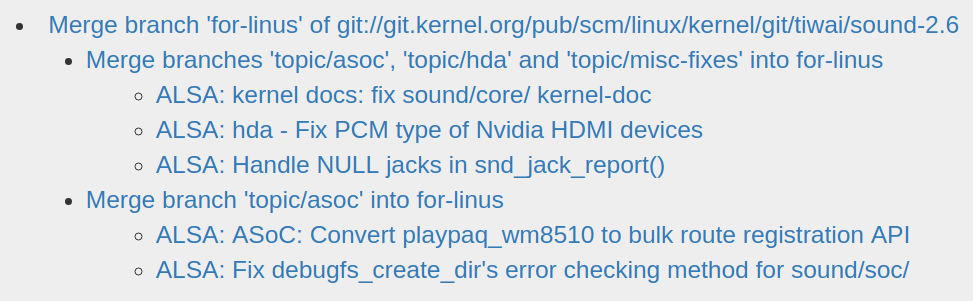
\includegraphics[width=0.9\figwidth]{figures/linvis/linvis_list_tree.png}
        \caption{The list tree visualization}
        \label{fig:linvis_list_tree}
\end{figure}

\subsubsection{\rt Tree}

The \rt tree\cite{Reingold1981}, depicted for two trees in
Figure~\ref{fig:study_commits}, is the classic tree visualization, with
the root at the top, leaves at the bottom, and edges between them
showing the parent-child relationship. This tree visualization works
very well in many cases, but does not easily visualize very wide trees,
with many repository events on a single level.

When a user first looks at the visualization, the current repository
event is placed in the center. Furthermore, it is highlighted in bright
orange. Commits, the leaves, are shown in white, while the merges are
colored shades of blue where lighter blue indicates fewer child events
of that node, and darker blue indicates more children.

\subsubsection{Pack Tree}

Pack trees\cite{Wang2006} are useful for displaying an overview of large
data sets. The initial goal for the pack tree was for visualizing file
systems, which are similar to git repositories in that they are
relatively shallow, but very wide trees. The tree is represented by sets
of nested circles. The largest circle, containing all of the other
nodes, is the root, while the smallest circles are the leaves. In our
representation, the root maps to the merge into the master branch, while
the leaves are the commits.


\begin{figure}[htpb]
  \centering
  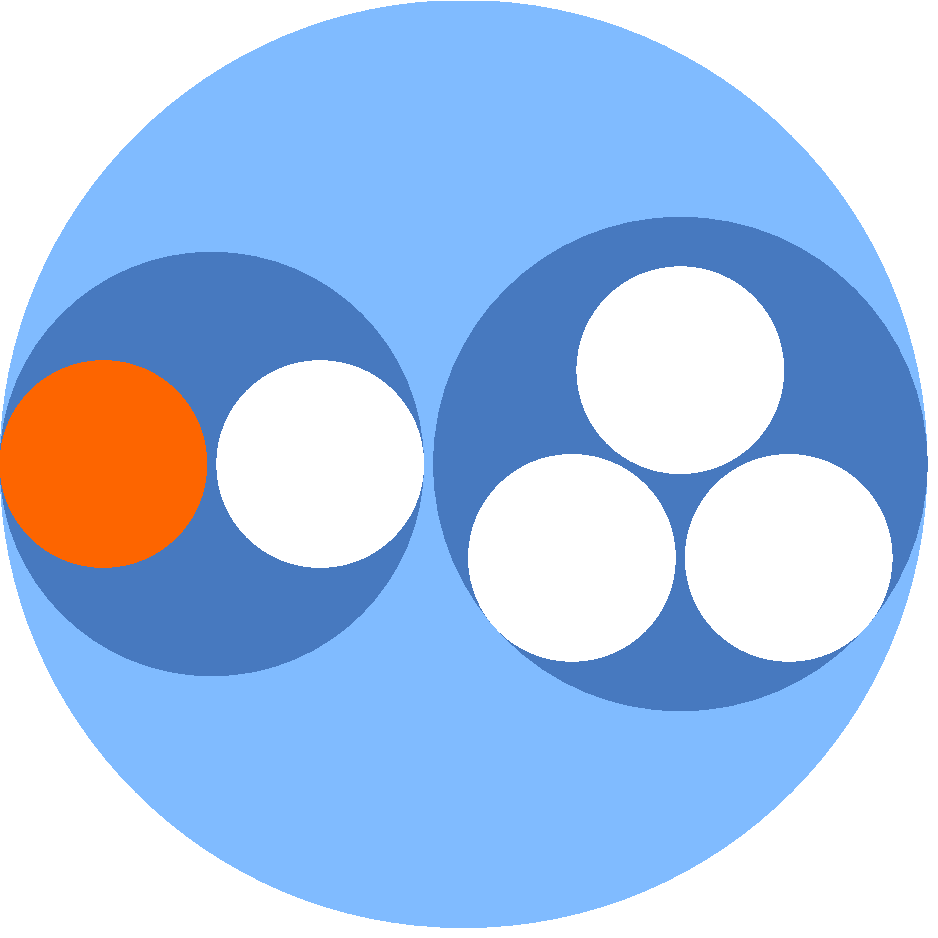
\includegraphics[width=0.8\figwidth]{figures/linvis/linvis_bubble.pdf}
  \caption{The pack tree visualization, with the root depicted as the
    outer-most circle, containing all other nodes, the leaves depicted
    as white circles containing no other nodes. The currently selected
    event is shown in orange.}
  \label{fig:linvis_pack}
\end{figure}

We depict the pack tree in Figure~\ref{fig:linvis_pack}. Like with the
\rt tree, \tool uses white to indicate the individual commits, and
orange to indicate the currently selected node. The inner merges are
colored with shades of blue to indicate the depth in the tree. Darker
shades of blue indicate that the merge is deeper in the tree; the root
will be the lightest shade.
